\documentclass[a4paper]{IEEEtran}

\usepackage{xcolor}
\usepackage{hyperref}
\usepackage[utf8]{inputenc}
\usepackage[pdftex]{graphicx} 

\newcommand\TODO[1]{\textcolor{red}{TODO:#1}}
\newcommand\todo[1]{\TODO{#1}}
\newcommand\cn{\textcolor{red}{[citation needed]}}

\title{Indiana Jones and the Quest for the Extraterrestrial Liaison!}

\author{
    Rune Holmgren,
    Torbjørn Langland
}

\begin{document}

\maketitle

\begin{abstract}
    \todo{ Compulsory (means that it is specified in the Term Project in description of report set up, and at this very location). Create a fitting abstract here. Also create a FRONT PAGE. Yes, you didn't read wrong. I wrote in capital letters. If we miss this now, we must indeed be quite stupid...}
\end{abstract}

\section{Front Page}
\todo{ Compulsory. Again, create FRONT PAGE. Didn't immediatly know better how to put this in, so just added this as first section (NOOB!). }

\section{Introduction}
\todo{ Compulsory. Introduction that explains what to expect of the report. Introduction of the term project should be covered in abstract? }

\section{Table of Contents}
\todo{ Compulsory. Must generate. I leave that to you, Rune}

\section{Problem to be solved. Method.}
\todo{ Insert chapter introduction here. }
\break
\subsection{Introduction}
This chapter will introduce the reader to the details of the problem that is to be solved through this Term Assignment. First the NTNU Student Satellite and the use need for a fault tolerant communication module will be described, then the Framework for the project will be detailed.

\subsection{The Liasion Fault Tolerant System}
NTNU is working with a Student Satellite, which is to orbit Earth and measure atmospheric data and deliver this to a ground stattion. The goal of this Assignment is to design a fault tolerant system called Liasion, which exploits redundancy. The system will contain four independent microcontrollers, that perform the same calculations. Every computation will procude 8-bit words. There is always the chance due to cosmic radiation that one more microcontrollers may produce incorrect data. If this is the case, the majority will decide the correct data, in a process known as \textit{voting}. The voted data is to be accompanied by a 3-bit status signal which contains the number of failed microcontrollers. If too many microcontrollers have failed, this status signal will indicate it so that recieved data cannot be trusted. Additionally, data may be corrupted before reaching Earth. This problem is to be solved by implementing a module with Error Correcting Circuit (ECC) that uses Hamming Code. The chosen solution must be able to correct single-bit errors and detect double-bit errors.
\break 
\todo{ Insert reference, this is from the introduction of the Term Assignment}
\paragraph{}
FIND A WAY TO REMOVE a)


\subsection{The Liasion Module functionality in details}
kkk

\subsection{Project Framework}
The system is to be encoded in VHDL, tested and verified in simulation, and synthesized, with a goal of having a few Look Up Tables (LUTs) as possible. \todo{ Perhaps briefly explain what a LUT is?}
Active HDL \todo{ Version number?} is used for programming in VHDL, as well as creating test benches and running simulations for verification. Synplify Pro \todo{ Version number?} is used for synthesizing, creating resulting LUTs and estimated frequency, and creating RTL schematics and Gate-Level \todo{ Find correct name} schematics. 
\break 
\todo{ Replace break with new paragraph in such a way that \textit{a)}, \textit{b)}, \textit{c)}, ... is not added}
\break
\todo{ Yes, new paragraph here} The Term Assignment was handed out at \todo{ Insert date here, somewhere in January}. These are the milestones: \todo{ Again, need reference from the Term Assignment}
\begin{itemize}
    \item February 18th, 2014: Assignment 3 of the Course, where the individual One-Bit Voters are designed. They serve as basis of the 8-bit voters
    \item February 28th, 2014: Delivery of technical notes, that will contain preliminary solutions to sub-problems 1, 2 and 3.
    \item March 3rd, 2014: Delivery of Peer Evaluation, containing evaluation of the technical note and project of another group.
    \item March 31st, 2014: Presentation of the project for groups 1-9 (minus 7).
    \item April 3rd, 2014: Presentation of the project for groups 7, 10-19.
    \item April 4th, 2014: Final report delivery.
\end{itemize}

\break
\break
\todo{ Describe the idea for the Liaison system. Treat it like a black box and explain what it is supposed to do.}
\break
\break
\todo{ Include figure(s) from pages 4-5 in order to explain the wanted functionality. }
\break
\break
\todo{ Also mention that the solution to this problem is split into different sub-sproblems? }

\section{ Solution to the problem}
\todo{ Term project specifies that the answer to all subproblems is to be explained. We should therefore split these into subsection. }
\break
\break
\todo{ Insert chapter introduction here. Remember to mention that we used Active HDL and Synplify Pro.}
\break
\break
\todo{ WARNING: Points of Term project report specifiaction sort of overlaps. Perhaps own chapters for testing and verification, or only the sub-chapters of this one are enough. Discuss, choose, live, rule, win!} 

\subsection{Sub-Problem 1: State analysis}
\todo{ Insert the State Machine figure here. Explain it, and choices the group has done in the design. }

\subsection{Sub-Problem 2: One-Bit voter}
\todo{ Explain the implementation of the One-bit Voter.}
\break 
\break
\todo{ Explain test results. Include figures. OR explain in section "Testing and verification" }
\break
\break
\todo{ Explain synthesis results: Estimated Frequency and generated LUTs}
\break
\break
\todo{ Find out if one or both voters must be explained (at least mention synthesis results of the second one). }

\subsection{Sub-Problem 3: 8-Bit voter}
\todo{ Explain the different options for implementations. Include figures. (Can screenshot from technical note. Yehaa, there was some use from that long night after all :P ) }
\break
\break
\todo{ Explain the chosen architecture. Include figure (screenshot it from the presentation). }
\break
\break
\todo{ Explain test results. Include figures. OR explain in section "Testing and verification" }
\break
\break
\todo{ Explain synthesis results}
\break
\break


TEXT
\begin{figure}[h!]
  \centering
      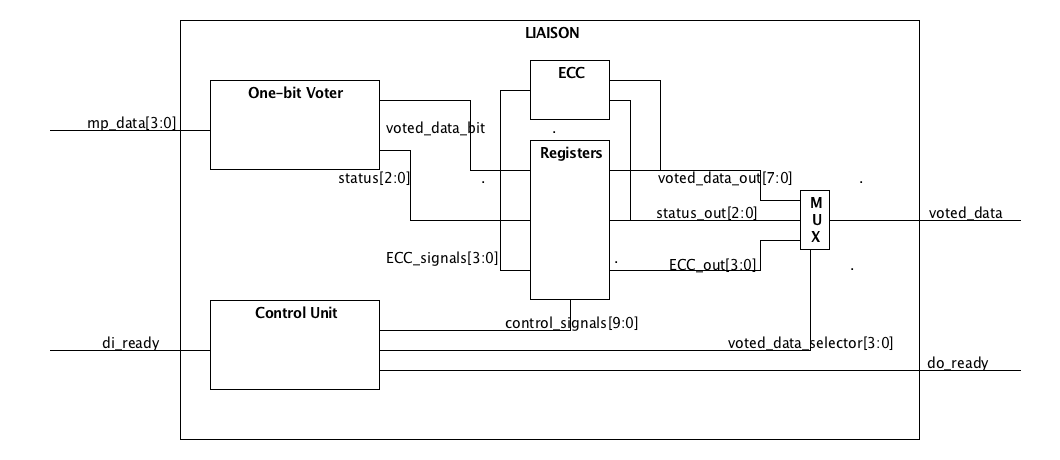
\includegraphics[width=0.5\textwidth]{Figures/ArchitectureFinal}
  \caption{Chosen architecture for the 8-bit Voter}
  \label{fig:ArchitectureFinal}
\end{figure}
TEXT
\begin{figure}[h!]
  \centering
      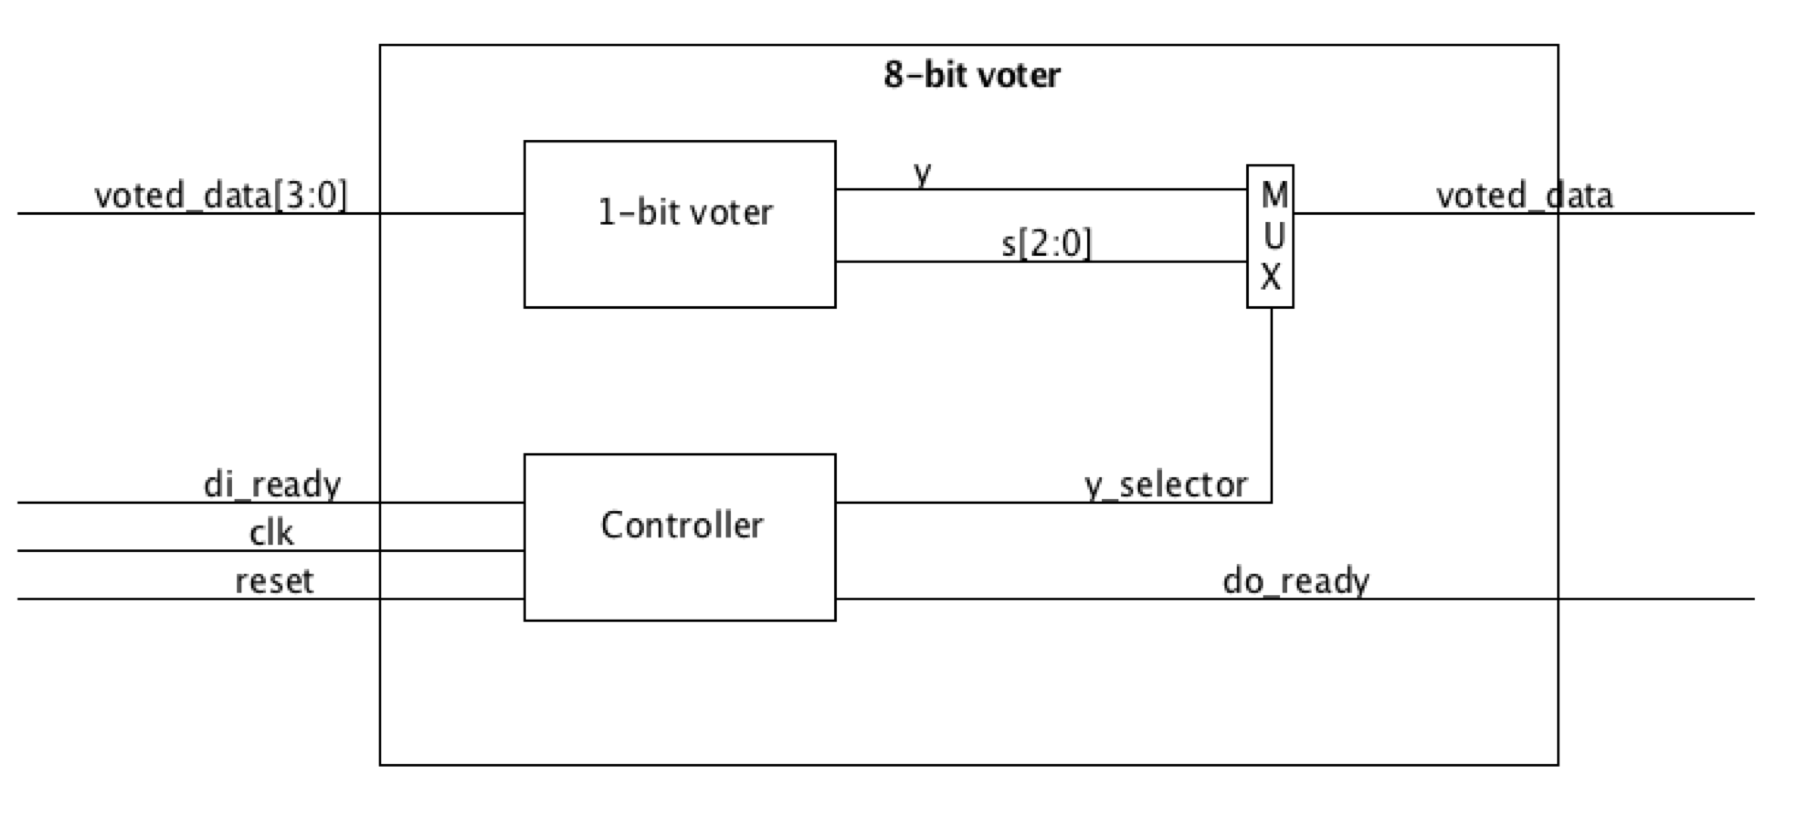
\includegraphics[width=0.5\textwidth]{Figures/ArchitectureOption2}
  \caption{Chosen architecture for the 8-bit Voter}
  \label{fig:ArchitectureOption2}
\end{figure}
TEXT
\begin{figure}[h!]
  \centering
      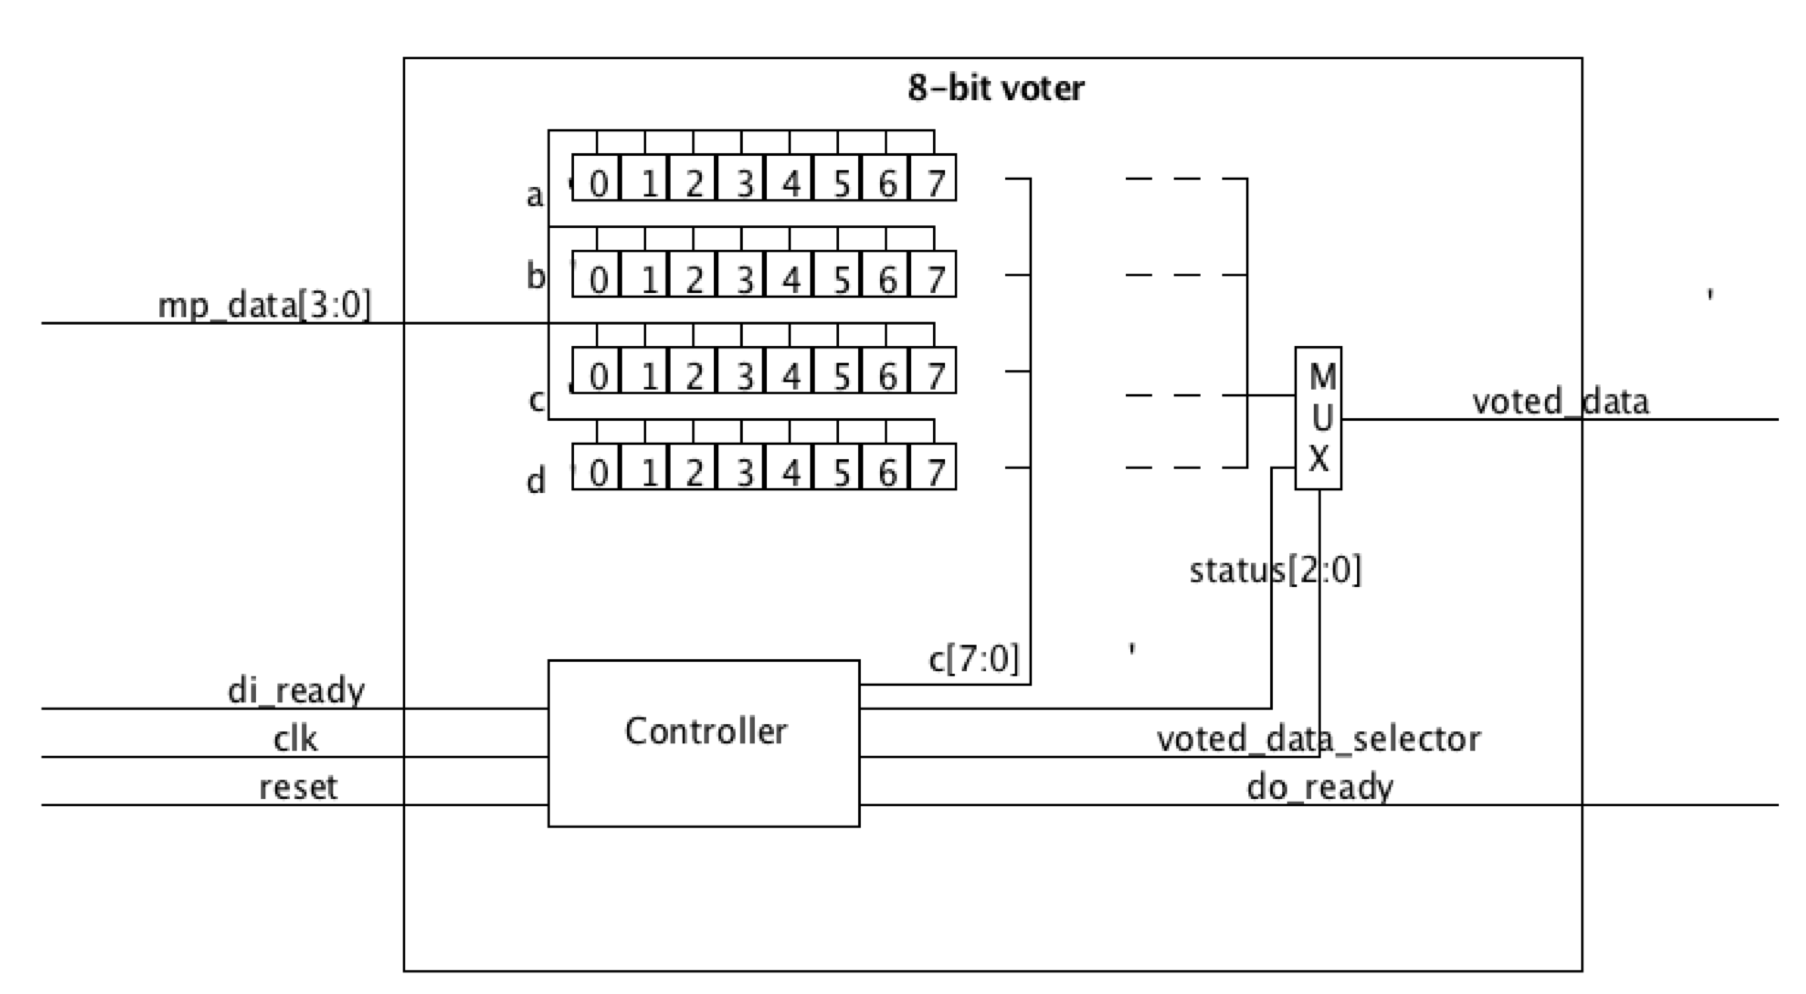
\includegraphics[width=0.5\textwidth]{Figures/ArchitectureOption3}
  \caption{Chosen architecture for the 8-bit Voter}
  \label{fig:ArchitectureOption3}
\end{figure}

TEXT
\subsubsection{ Details of the 8-bit voter}.
\todo{ Detail the controller.}
\break
\break
\todo{ Detail the Registers.}
\break
\break
TEXT
\begin{figure}[h!]
  \centering
      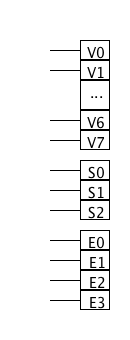
\includegraphics[width=0.5\textwidth]{Figures/Registers}
  \caption{Chosen architecture for the 8-bit Voter}
  \label{fig:Registers}
\end{figure}

\subsection{Sub-Problem 4: Error Correction Circuit}
\todo{ Explain how the ECC is implemented, perhaps explain Hamming Coding. Include figure (screenshot it from the presentation). }
\break
\break
\todo{ The term project states: "Your final report should comment on the use of intellectual property-modules and the reasoning behind why this scheme is appropriate." To this.}
\break
\break
\todo{ Explain test results. Include figures. OR explain in section "Testing and verification" }
\break
\break
\todo{ Explain synthesis results}

\subsection{Sub-Problem 5: Analysis of error probabilities}
\todo{ Explain briefly the theory behind a microcontroller failure. }
\break
\break
\todo{ Explain the mathematical expressions for P(Max(1)), P(Max(2)), P(Least(3), and the results from calculating MTTF.}
\break
\break
\todo{ Refer to Appendix C for full calculation.}

\section{ Testing and verification }
\todo{ Either explein the testing and verification here, or do it seperately in the subchapters of the previous chapter. Delete this chapter if we choose the other solution. I vote this one. But if we do so, for consistensy we may then have to create a independent chapter for Synthesis }
\break
\break
\todo{ Insert introduction }

\subsection{ Tests and verification of One-Bit Voter}
\todo{ Explain choice of test bench. Explain why it gives full coverage}
\break
\break
\todo{ Explain test results. Include screenshot (Uh... the provided test bench is not of that kind).}

\subsection{ Control Unit}
\todo{ Explain choice of test bench. Explain why it gives full coverage}
\break
\break
\todo{ Explain test results. Include screenshot. }

\subsection{ ECC }
\todo{ Explain choice of test bench. Explain why only partial coverage is enough. }
\break
\break
\todo{ Explain test results. Include screenshot. }

\subsection{ Liasion }
\todo{ Explain choice of test bench. Explain why only partial coverage is enough. }
\break
\break
\todo{ Explain test results. Include figure. (Screenshot it from the presentation) }

\section{Synthesis }
\todo{ Decide whether we should have a own chapter for this or not. If we choose this option for testing and verification, we should do this for synthesis as well in the name of consistency. }
\break
\break
\todo{ Insert introduction }
\break
\break
\todo{ Refer to Appendix B for schematics. Both RTL and that other one. }


\section{Conclusion}
\todo{ Compulsory. Have a good wrap up, somehow. }

\section{Acknowledgements (optional)}

Indiana Jones. Should also mention group 2 and the student assistant.

\section{ Other problems/needs to be solved:}
\subsection{ Appendixes}
\todo{ Appendix A: Project codes }
\break
\break
\todo{ Appendix B: Synthesis Schematics. Both RTL and that other type, propose top architecture first then One-bit-Voter, Controller, Registers and ECC. RTL first then that other type.}
\break
\break
\todo{ Appendix C: The Probability Calculation. I got it covered. }
\subsection{ Other problems/needs:}
\todo{ Find out where to list up time spent in the project.}

\bibliographystyle{plain}
\nocite{*}

\end{document}
